% H2 progress: per-window editing strength (mu) and return multiplier (alpha) for GTA
% Compile: tectonic h2_progress.tex   (or pdflatex twice, or upload this folder to Overleaf)
\documentclass[aspectratio=169,11pt]{beamer}
\usepackage[T1]{fontenc}
\usepackage{amsmath,amssymb,booktabs,graphicx,tabularx,xcolor,array}
\graphicspath{{figures/}{/home/da25d400/arl_proj/rarl-proj/docs/h2_progress/figures/}}

% Style matched to the HSM/HiPER weekly-meet deck: blue title bars, blue title box, plain footline
\usetheme{default}
\usefonttheme{professionalfonts}
\setbeamertemplate{navigation symbols}{}
\definecolor{bar}{HTML}{3333B3}
\definecolor{bardark}{HTML}{23238A}
\definecolor{blockbody}{HTML}{E9EAF6}
\definecolor{acc}{HTML}{3333B3}
\definecolor{ok}{HTML}{1F6F43}
\definecolor{no}{HTML}{D01010}
\setbeamercolor{structure}{fg=bar}
\setbeamercolor{frametitle}{fg=white,bg=bar}
\setbeamercolor{title}{fg=white,bg=bar}
\setbeamercolor{block title}{fg=white,bg=bardark}
\setbeamercolor{block body}{fg=black,bg=blockbody}
\setbeamercolor{block title alerted}{fg=red,bg=}
\setbeamercolor{block body alerted}{fg=black,bg=}
\setbeamerfont{frametitle}{size=\Large}
\setbeamerfont{title}{size=\Large}
\setbeamertemplate{itemize items}[triangle]
\setbeamertemplate{enumerate items}[default]
\setbeamertemplate{blocks}[default]
\setbeamertemplate{frametitle}{%
  \nointerlineskip
  \begin{beamercolorbox}[wd=\paperwidth,ht=2.6ex,dp=1.4ex,leftskip=0.6em]{frametitle}
    \usebeamerfont{frametitle}\insertframetitle
  \end{beamercolorbox}\vspace{0.4em}}
\setbeamertemplate{title page}{%
  \vfill
  \begin{beamercolorbox}[wd=\textwidth,sep=10pt,center]{title}
    \usebeamerfont{title}\inserttitle\par\vspace{0.2em}
    \normalsize\insertsubtitle
  \end{beamercolorbox}\vspace{2em}
  \begin{center}
    \large\insertauthor\par\vspace{1em}
    \footnotesize\insertinstitute\par\vspace{1.2em}
    \large\insertdate
  \end{center}\vfill}
\setbeamertemplate{footline}{%
  \hspace{0.6em}\scriptsize\color{darkgray}\insertshorttitle\hfill
  \insertframenumber/\inserttotalframenumber\hspace{6em}\vspace{0.8em}}
\newcommand{\hyp}[1]{\textcolor{acc}{\textbf{#1}}}
\newcommand{\yes}{\textcolor{ok}{\textbf{supported}}}
\newcommand{\nope}{\textcolor{no}{\textbf{not supported}}}
\newcommand{\cond}[1]{\texttt{#1}}
\newcolumntype{Y}{>{\raggedright\arraybackslash}X}

\title[GTA $\rightarrow$ per-window $\mu$, $\alpha$ $\rightarrow$ results so far]{Per-window Editing in GTA: Support-based $\mu$ and $\alpha$}
\subtitle{H2 study on halfcheetah-medium-v2, the reconstruction-score support, and follow-up tests H3--H7}
\author{Karan Kishore}
\institute{IIT Madras}
\date{Weekly Meet \,$|$\, October 26, 2026}

\begin{document}

\begin{frame}
\titlepage
\end{frame}

% ---------------------------------------------------------------------------------------------
\begin{frame}[shrink=18]{Summary}
\small
\textbf{GTA} edits every trajectory window with one global noising ratio $\mu$ and one return multiplier $\alpha$.
We asked whether these should be chosen \emph{per window}.
\vspace{0.4em}

\renewcommand{\arraystretch}{1.15}
\begin{tabularx}{\linewidth}{@{}p{0.33\linewidth}Yp{0.13\linewidth}@{}}
\toprule
test & result & verdict\\
\midrule
H2a: more support $\Rightarrow$ higher safe $\mu$ & $\mu^{\text{safe}}$ rises $+0.18$ $[0.14,0.23]$ from lowest to highest support & \yes\\
H2b: higher quality $\Rightarrow$ lower $\mu$ & $\beta_Q\approx0$; quality only predicts reward gain & \nope\\
H2c: support-adaptive $\mu$ (mean 0.3) & $+3.4$ over uniform 0.3, $+3.1$ over inverted (JAX) & \yes\\
H2c-wide: adaptive $\mu$ (mean 0.5) & $-0.7$ vs uniform 0.5 ($p=0.20$) & \nope\\
$\alpha$ by support & $\alpha_{\text{up}}$ $+0.9$ over $\alpha=1.3$, but $=$ random mix ($p=0.35$) & not specific\\
Learned $\mu(S,Q),\alpha(S,Q)$ (CMA-ES) & $58.76$ vs $59.05$ for tuned global ($p=0.29$) & \nope\\
\bottomrule
\end{tabularx}
\vspace{0.4em}

\textbf{Bottom line:} support reliably predicts \emph{how much physics damage} an edit does; turning that into a better RL score
only helps when $\mu$ is small. At GTA's own operating point ($\mu=0.5$, $\alpha=1.3$) a single well-tuned global setting is as good.
\end{frame}

\begin{frame}{Outline}
\begin{enumerate}
\item Setup: GTA editing, $\mu$ and $\alpha$
\item H2 made measurable: quality $Q$ and three support metrics, including the \textbf{reconstruction score} $S_2$
\item Window-level study: pilot ($S_1$) $\to$ main ($S_2$)
\item Assigning $\mu$ by support: Experiment A (PyTorch and JAX TD3+BC), narrow and wide mappings
\item Assigning $\alpha$ by support: global sweep, up/down, random-mix control
\item Learning continuous $\mu(S,Q)$ and $\alpha(S,Q)$ with CMA-ES
\item Follow-up tests H3--H7 (no-generation baselines, VAE editors, trust weighting, bound)
\item Limitations and next steps
\end{enumerate}
\end{frame}

% =============================================================================================
\section{Setup}
\begin{frame}{GTA in one slide (Lee et al., NeurIPS 2024)}
\begin{enumerate}
\item \textbf{Train:} a conditional diffusion model (MixerUnet, 29.6M params, EDM, 1M steps) learns $32\times24$ trajectory windows given their return.
\item \textbf{Edit:} take a real window $\tau^0$, noise it once to level $\sigma(\mu K)$, then denoise for $\mu K$ steps conditioned on the \emph{amplified} return $\alpha\cdot\text{RTG}$.
\item \textbf{Train RL:} add edited windows (as transitions) to the 1M original transitions; train TD3+BC.
\end{enumerate}
\vspace{0.5em}
\begin{tabularx}{\linewidth}{lY}
\toprule
$\mu\in(0,1]$ & how much of the window is rewritten (exploration). Paper: $\mu=0.5$\\
$\alpha>1$ & how hard the edit is pushed to higher reward (exploitation). Paper: $\alpha=1.3$\\
$K$ & 128 noise levels; $\mu$ is very non-linear in noise: $\sigma=0.16$ at $\mu=0.25$, $2.43$ at $\mu=0.5$\\
\bottomrule
\end{tabularx}
\vspace{0.5em}

Data: D4RL \texttt{halfcheetah-medium-v2}, 1{,}000 episodes $\times$ 1{,}000 steps. Guidance $w=0$ (config temperature 1).
\end{frame}

\begin{frame}{Sanity check: GTA edits on random windows}
\begin{columns}[T]
\begin{column}{0.55\linewidth}
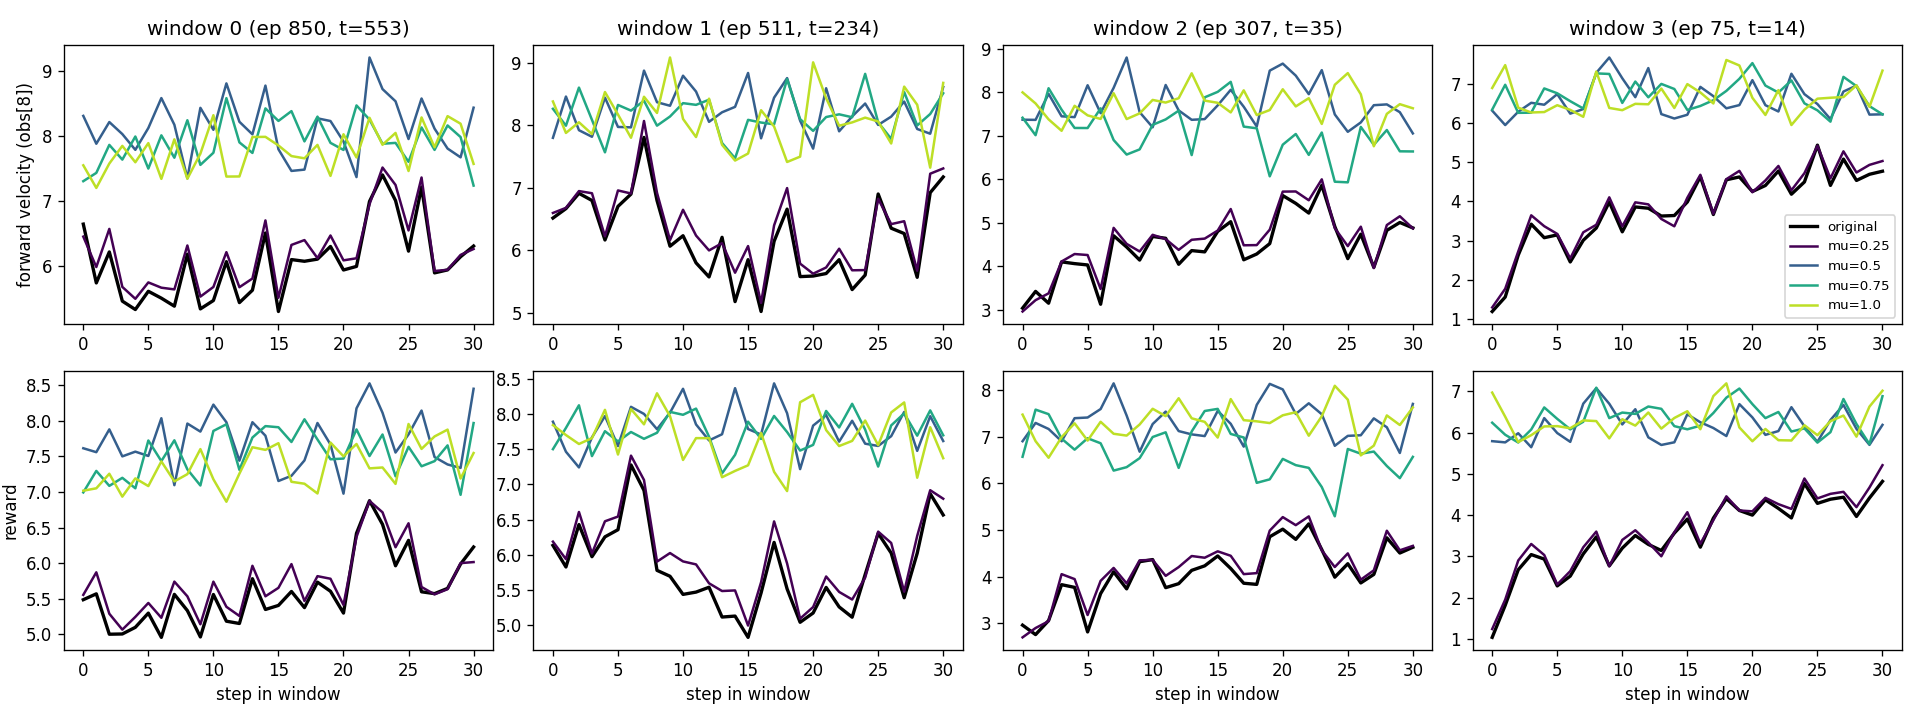
\includegraphics[width=\linewidth]{demo_mu_sweep.png}

\scriptsize Top: forward velocity; bottom: reward over 31 steps. Black = original.
\end{column}
\begin{column}{0.43\linewidth}
\begin{itemize}
\item $\mu=0.25$: almost no change ($+3\%$ reward).
\item $\mu\ge0.5$: $+35$--$75\%$ reward while staying physically valid in MuJoCo.
\item Model-written reward matches the simulator within 0.5.
\end{itemize}
\vspace{0.5em}
Every edit is replayed in MuJoCo to get the true reward (\texttt{oracle\_r}), physics error (\texttt{dyn\_mse}, paper Eq.~11) and distance from source (\texttt{shift}).
\end{column}
\end{columns}
\end{frame}

% =============================================================================================
\section{Measuring H2}
\begin{frame}{The hypothesis}
\hyp{H2.} The best $\mu$ for a window depends on two of its properties:
\begin{itemize}
\item \hyp{H2a (support):} better covered by the data $\Rightarrow$ \textbf{higher} $\mu$ is safe.
\item \hyp{H2b (quality):} higher own reward $\Rightarrow$ \textbf{lower} $\mu$.
\item \hyp{H2c (downstream):} choosing $\mu$ per window from support improves TD3+BC.
\end{itemize}
\vspace{0.6em}
\textbf{Quality:} $q_i=\sum_{t=0}^{30}0.99^t r_{t}$ inside the window; $Q_i$ = percentile rank.
\vspace{0.3em}

\textbf{Support:} three implementations, from data-only to model-based to exact:
\begin{center}
\begin{tabular}{llll}
\toprule
 & what it measures & cost & role\\
\midrule
$S_1$ & kNN distance in $(s,a)$ space & cheap & pilot\\
$S_2$ & diffusion \textbf{reconstruction score} & 12 network calls & \textbf{primary}\\
$S_3$ & exact log-likelihood (prob.-flow ODE) & very slow & validation\\
\bottomrule
\end{tabular}
\end{center}
\end{frame}

\begin{frame}{Support $S_1$: nearest neighbours in the data}
\begin{enumerate}
\item Standardise every $(s,a)\in\mathbb R^{23}$ over all 1M transitions.
\item For each step $t$: distance to the \textbf{20th nearest} transition from a \textbf{different episode}
\[
d_{20}(j_t)=\text{20th smallest of }\{\lVert z_{j_t}-z_{j'}\rVert_2:\ \text{ep}(j')\neq\text{ep}(j_t)\}.
\]
\item $\text{s1\_dist}_i=\operatorname{median}_t d_{20}(j_t)$; $S_{1,i}$ = percentile rank of $-\text{s1\_dist}_i$.
\end{enumerate}
\vspace{0.4em}
\begin{itemize}
\item kNN density: $\hat p(x)\propto 1/d_k(x)^{23}$ --- smaller distance, denser region. Inverse of GTA's \emph{novelty} metric.
\item Same-episode neighbours are excluded (adjacent steps are near-identical).
\item Limitation: ignores the trained model; says nothing about what the \emph{diffusion model} finds familiar.
\end{itemize}
\end{frame}

\begin{frame}{Support $S_2$: the reconstruction score}
\begin{enumerate}
\item Normalise the window $\tilde x$. For $\sigma\in\{0.16,0.5,2.4\}$ and 4 noise draws, one \emph{unconditional} denoiser call:
\[
\hat x=D_\theta(\tilde x+\sigma\varepsilon_n;\ \sigma,\varnothing)
\]
\item Masked reconstruction error $e_i(\sigma)=\tfrac14\sum_n \lVert M\odot(\hat x-\tilde x)\rVert^2/\textstyle\sum M$.
\item $\text{s2\_score}_i=-\operatorname{mean}_\sigma\ z\text{-score}_{\text{pool}}\big(\ln e_i(\sigma)\big)$; \quad $S_{2,i}$ = percentile rank.
\end{enumerate}
\vspace{0.4em}
\textbf{Why it measures support:}
$-\log p(x)\le\int w(\sigma)\,\mathbb E_\varepsilon\lVert D_\theta(x+\sigma\varepsilon;\sigma)-x\rVert^2d\sigma+C$
(Kingma et al.\ 2021; Song et al.\ 2021). $S_2$ is a 3-point estimate of this bound.
\vspace{0.3em}

\begin{itemize}
\item The three $\sigma$ are exactly the noise levels an edit uses at $\mu\approx0.25,0.35,0.5$: it asks \emph{``can the model rebuild this window from the noise it will actually get?''}
\item Cheap enough for all 161k windows used in RL experiments.
\end{itemize}
\end{frame}

\begin{frame}{Support $S_3$ and agreement of the three metrics}
\small
$S_3$: exact $\log p_0(x)$ via the probability-flow ODE with Hutchinson divergence (dopri5); 100 windows only.
\vspace{0.4em}

\begin{columns}[T]
\begin{column}{0.42\linewidth}
\centering
\begin{tabular}{lr}
\toprule
pair & Spearman $\rho$\\
\midrule
$S_1$ vs $S_2$ (20k) & 0.79\\
$S_2$ vs $S_3$ (100) & 0.74\\
$S_1$ vs $S_3$ (100) & 0.83\\
$Q$ vs $S_1$ & 0.49\\
$Q$ vs $S_2$ & 0.42\\
\bottomrule
\end{tabular}
\end{column}
\begin{column}{0.56\linewidth}
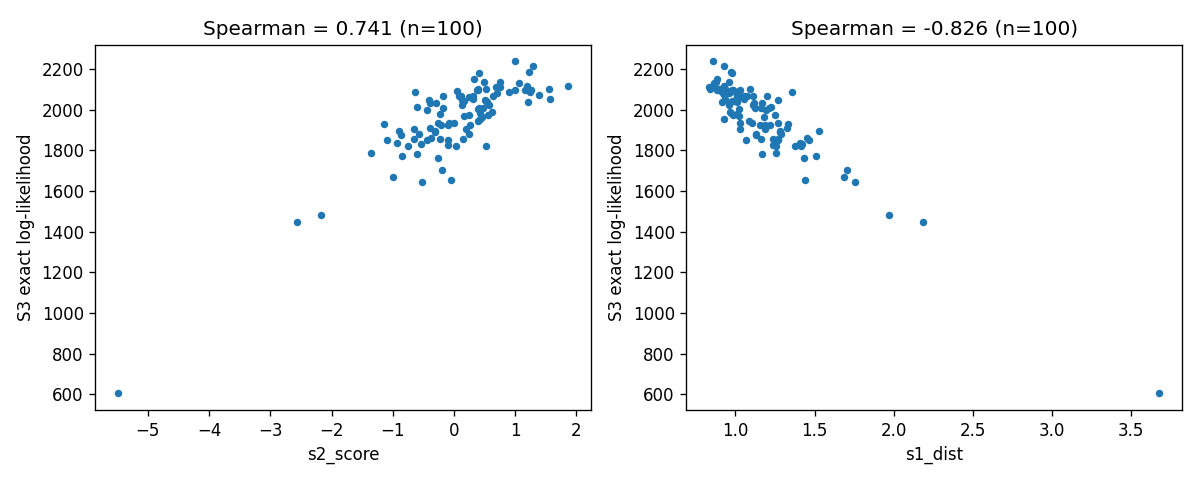
\includegraphics[width=\linewidth]{main_pool_s3_check.png}
\end{column}
\end{columns}
\vspace{0.4em}
\begin{itemize}
\item Data-based and model-based support agree and both track the exact likelihood.
\item Support and quality are related but separable $\Rightarrow$ stratified $5\times5$ design on $Q\times S$.
\end{itemize}
\end{frame}

\begin{frame}{From edits to ``the best $\mu$'' of a window}
\small
For window $i$, with gain and physics error on the $\mu$ grid and threshold $\theta=0.0085$ (paper's mean dyn.\ MSE):
\begin{itemize}
\item $\mu^*_i=\arg\max\{\text{gain}_i(\mu):\ \text{dyn}_i(\mu)\le\theta\}$ \hfill best reward among valid edits
\item $\mu_{90,i}=\min\{\mu:\ \text{gain}_i(\mu)\ge0.9\max\text{gain}_i\}$ \hfill how much editing it needs
\item $\mu^{\text{safe}}_i$ = largest $\mu$ before $\text{dyn}_i$ first exceeds $\theta$ \hfill how far it can be pushed safely
\end{itemize}
\vspace{0.3em}
\textbf{Statistics} ($n=400$ windows):
\[
y_i=\beta_0+\beta_Q(Q_i-\tfrac12)+\beta_S(S_i-\tfrac12)+\beta_{QS}(Q_i-\tfrac12)(S_i-\tfrac12)+e_i
\]
95\% CI: 2{,}000 bootstrap resamples; $p$: 2{,}000 permutations.
\vspace{0.3em}

\textbf{Decision rule (fixed in advance):} \yes{} if CI($\beta_S$)$>0$, CI($\beta_Q$)$<0$ and the extreme-quadrant gap $\ge0.1$.
\end{frame}

% =============================================================================================
\section{Window-level study}
\begin{frame}[shrink=3]{Pilot ($S_1$, 184 windows): ceiling effect hid support}
\begin{columns}[T]
\begin{column}{0.42\linewidth}
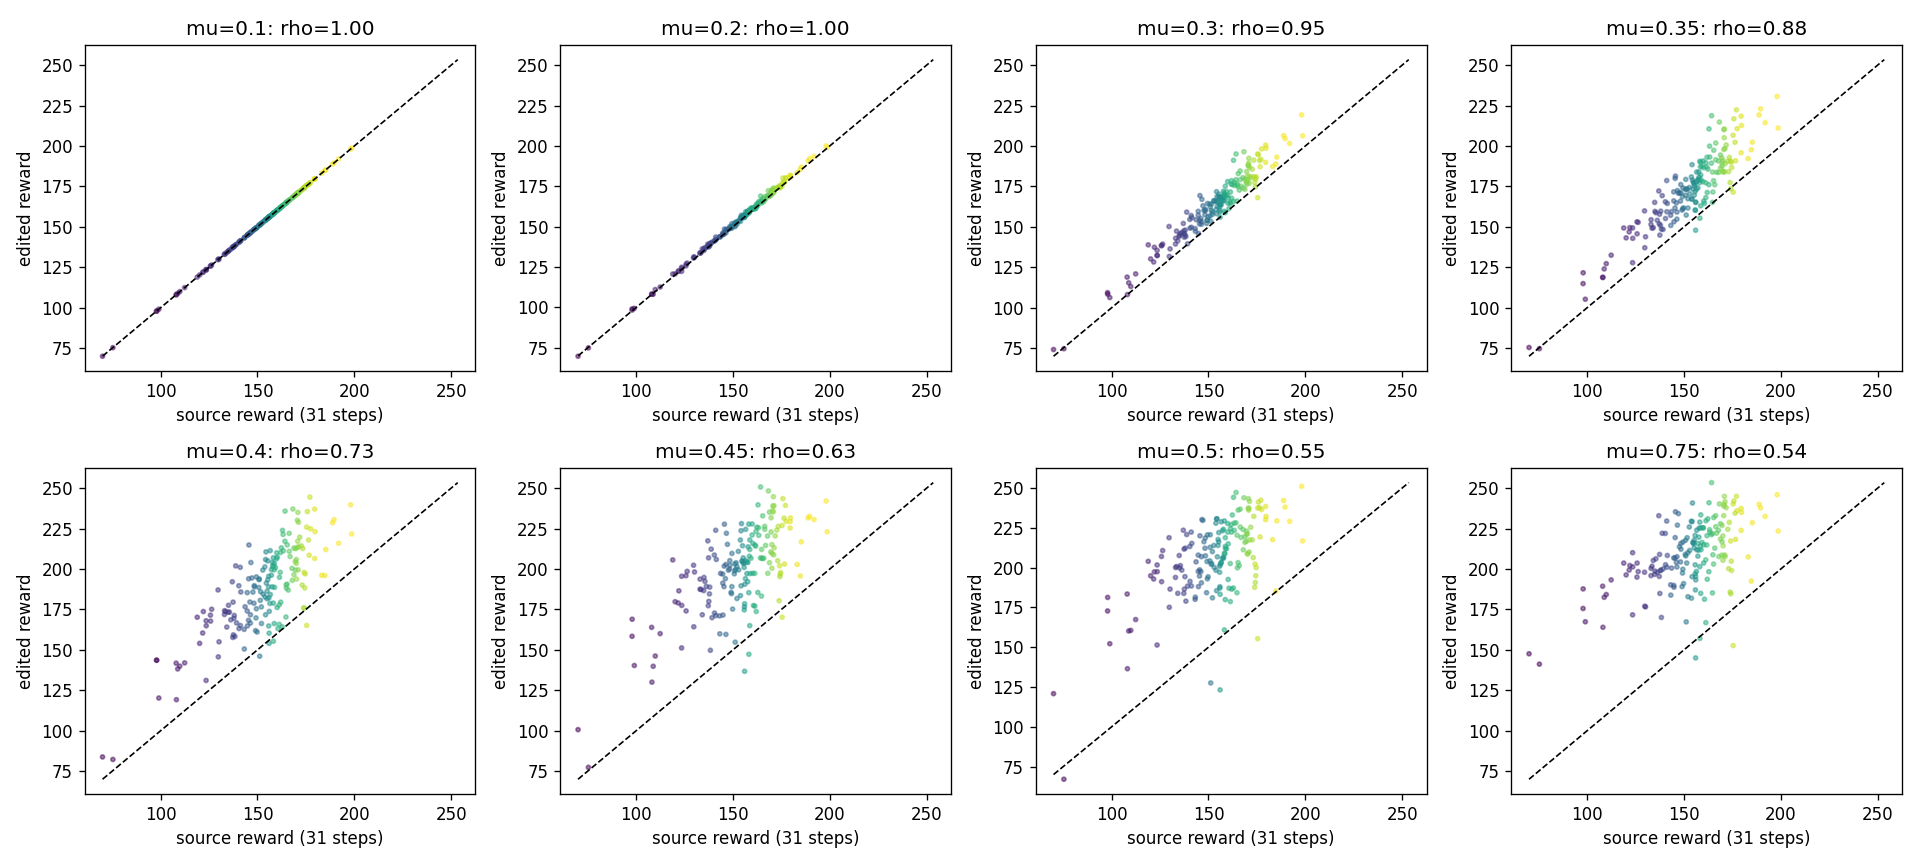
\includegraphics[width=\linewidth]{pilot_ceiling.png}

\scriptsize At $\mu\ge0.45$ edits converge to $\approx175$--$250$ reward whatever the source.
\end{column}
\begin{column}{0.56\linewidth}
\scriptsize
\begin{tabular}{@{}lll@{}}
\toprule
$\mu^*$ analysed with & $\beta_Q$ [95\% CI] & $\beta_S$ [95\% CI]\\
\midrule
all $\mu$, $\theta=0.017$ & $-0.17$ $[-0.24,-0.10]$ & $+0.02$ $[-0.05,0.09]$\\
all $\mu$, $\theta=0.0085$ & $-0.15$ $[-0.22,-0.08]$ & $-0.01$ $[-0.08,0.07]$\\
$\mu\le0.5$, $\theta=0.017$ & $-0.02$ $[-0.05,0.00]$ & $+0.01$ $[-0.02,0.05]$\\
$\mu\le0.5$, $\theta=0.0085$ & $-0.01$ $[-0.05,0.02]$ & $\mathbf{+0.09}$ $[0.04,0.14]$\\
\bottomrule
\end{tabular}
\vspace{0.5em}
\small
\begin{itemize}
\item The apparent quality effect came from $\mu=0.75$ edits that rewrite everything.
\item Restricting to $\mu\le0.5$ reveals a support effect.
\item \textbf{Fixed for main run:} $\mu\le0.5$, $\theta=0.0085$, support $S_2$.
\end{itemize}
\end{column}
\end{columns}
\end{frame}

\begin{frame}[shrink=14]{Main study ($S_2$): data funnel}
\centering\small
\begin{tabular}{@{}lrl@{}}
\toprule
stage & count & how\\
\midrule
transitions & 1{,}000{,}000 & 1{,}000 episodes $\times$ 1{,}000\\
eligible windows (start $\le800$) & 801{,}000 & RTG not truncated\\
pool & 20{,}000 & random; $Q$, $S_1$, $S_2$ computed ($S_3$ on 100)\\
selected windows & \textbf{400} & $5\times5$ grid on $Q\times S_2$ quintiles, 16 per cell\\
edits analysed & \textbf{5{,}600} & $400\times7\ \mu\ (\le0.5)\times2$ draws\\
simulated transitions & 198{,}400 & every edit replayed in MuJoCo\\
\bottomrule
\end{tabular}
\vspace{0.5em}

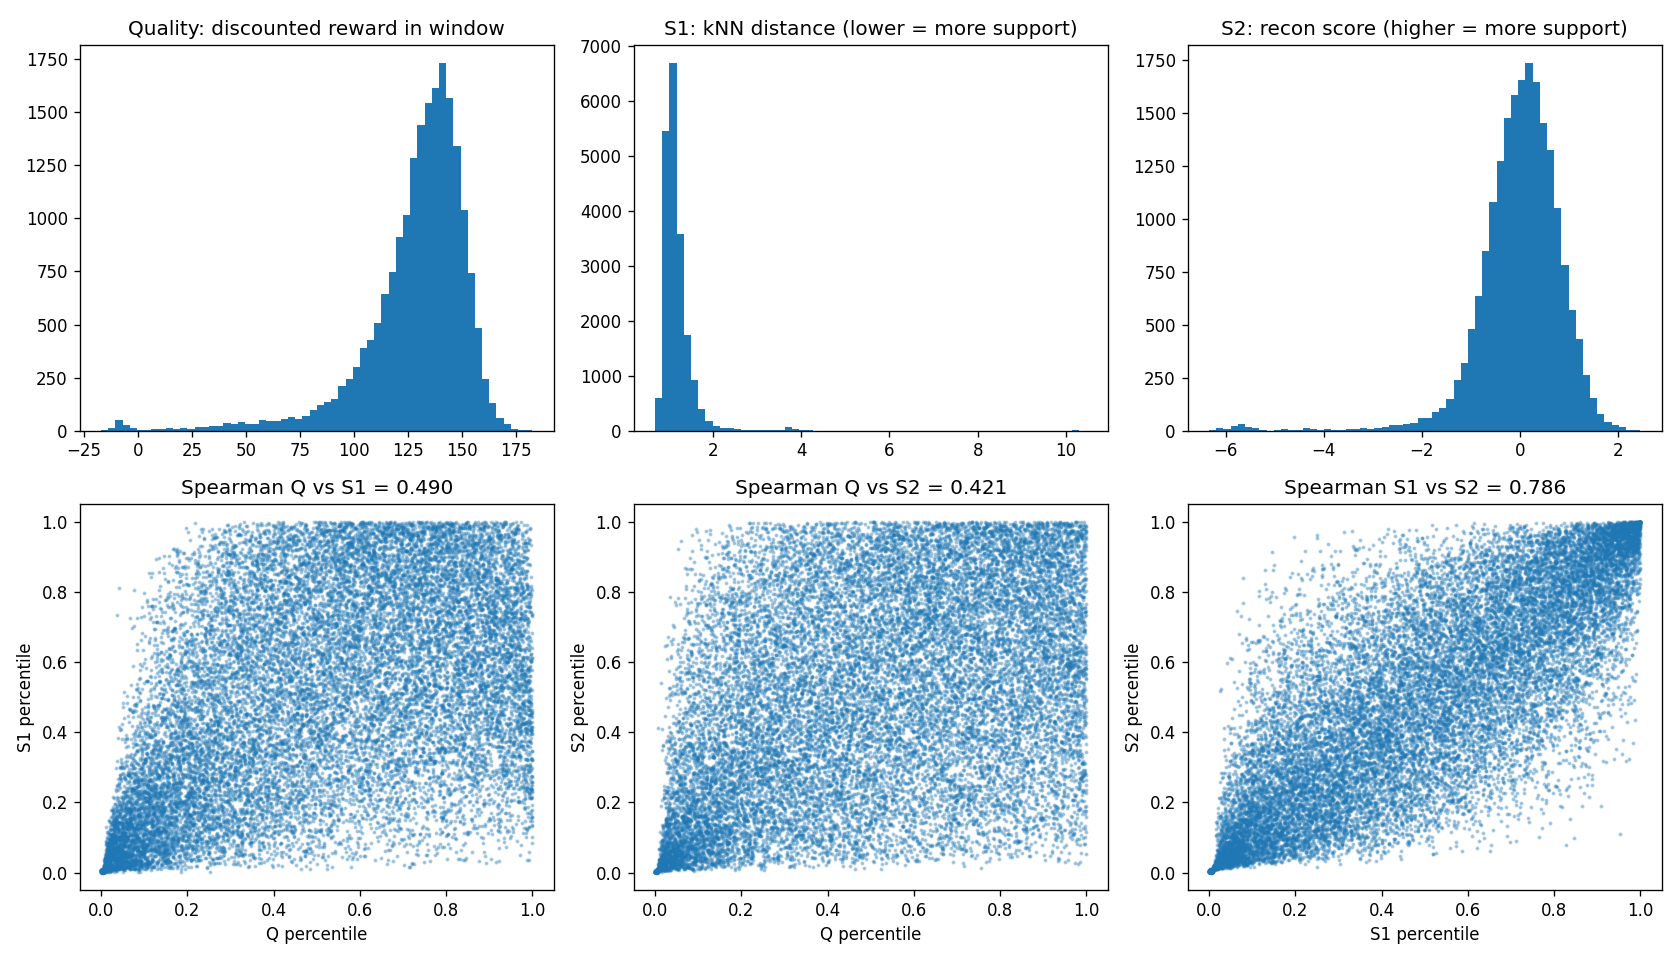
\includegraphics[width=0.6\linewidth]{main_pool_overview.png}
\end{frame}

\begin{frame}{Main result: gain follows quality, physics error follows support}
\centering
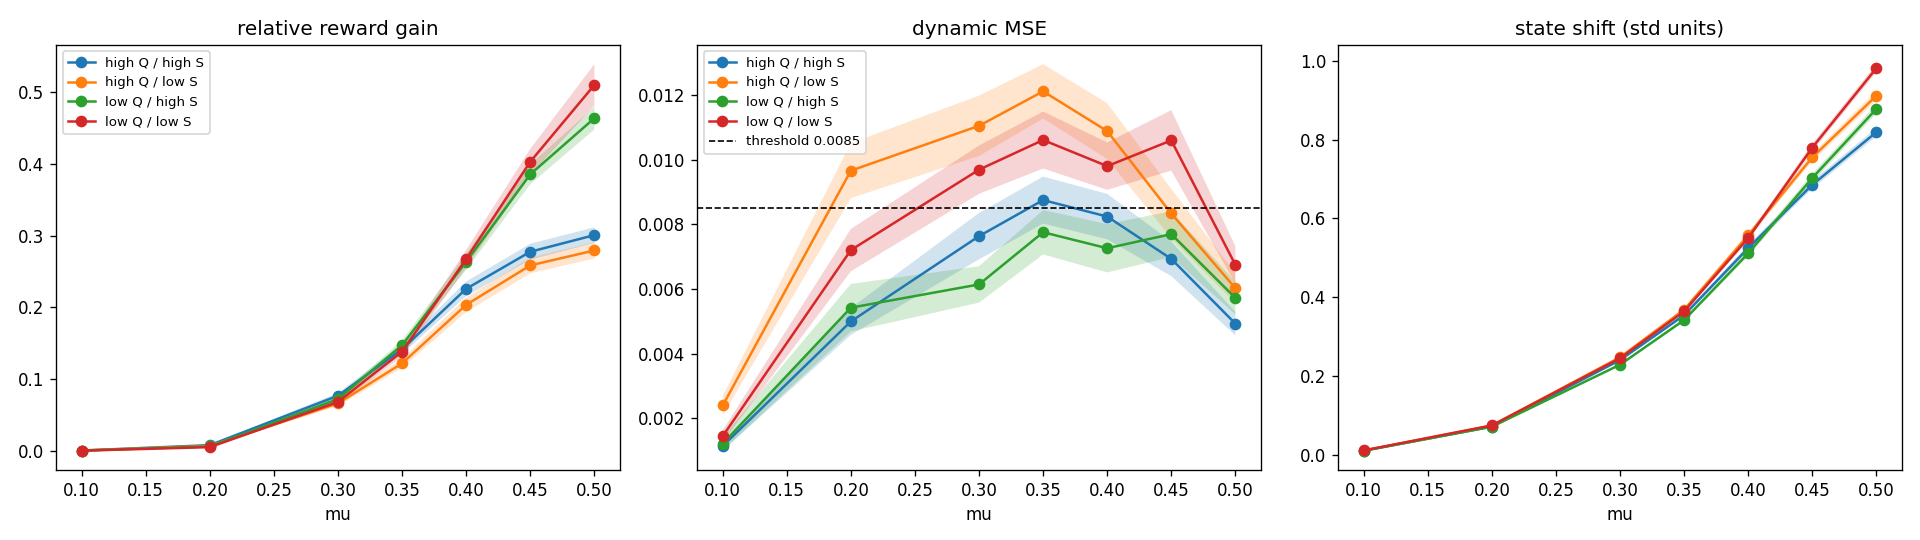
\includegraphics[width=\linewidth]{main_quadrant_curves.png}

\raggedright\small
\begin{itemize}
\item \textbf{Reward gain} rises with $\mu$ for all; low-$Q$ windows gain most (ceiling effect).
\item \textbf{Physics error} is higher for \emph{low-support} windows at every $\mu$, peaking at $\mu\approx0.35$.
\item \textbf{Shift} is the same for all quadrants: equal edit size, unequal damage.
\end{itemize}
\end{frame}

\begin{frame}{Correlations at every $\mu$ (Spearman, 400 windows)}
\centering
\small
\begin{tabular}{lrrrrrrr}
\toprule
$\mu$ & 0.1 & 0.2 & 0.3 & 0.35 & 0.4 & 0.45 & 0.5\\
\midrule
$S_2$ vs physics error & $-0.29$ & $-0.36$ & $-0.34$ & $-0.28$ & $-0.24$ & $-0.18$ & $-0.13$\\
$S_1$ vs physics error & $-0.25$ & $-0.34$ & $-0.32$ & $-0.26$ & $-0.28$ & $-0.25$ & $-0.15$\\
$Q$ vs physics error & $+0.07$ & $+0.01$ & $+0.01$ & $+0.09$ & $+0.04$ & $-0.14$ & $-0.07$\\
\midrule
$S_2$ vs reward gain & $+0.11$ & $+0.11$ & $+0.12$ & $+0.14$ & $+0.09$ & $+0.06$ & $+0.06$\\
$Q$ vs reward gain & $+0.13$ & $+0.17$ & $+0.01$ & $-0.11$ & $-0.25$ & $-0.51$ & $-0.65$\\
\midrule
mean reward gain & 0.000 & 0.007 & 0.071 & 0.138 & 0.240 & 0.331 & 0.388\\
mean physics error & 0.0015 & 0.0068 & 0.0086 & 0.0098 & 0.0090 & 0.0084 & 0.0058\\
share over $\theta$ & 0.02 & 0.24 & 0.36 & 0.43 & 0.41 & 0.33 & 0.18\\
\bottomrule
\end{tabular}
\vspace{0.6em}

\raggedright
Both support metrics predict physics error at every $\mu$; quality does not. Note the support effect \textbf{fades towards $\mu=0.5$}: at high noise the model regenerates the window and forgets the source.
\end{frame}

\begin{frame}{Test of H2 at window level}
\centering
\footnotesize
\begin{tabular}{@{}llllll@{}}
\toprule
outcome & $\beta_S$ [95\% CI] & $p_S$ & $\beta_Q$ [95\% CI] & gap & verdict\\
\midrule
$\mu^*$ & $+0.059$ $[0.030,0.090]$ & $<0.001$ & $-0.001$ $[-0.025,0.022]$ & $+0.034$ & S only, small\\
$\mu_{90}$ & $-0.002$ $[-0.014,0.009]$ & 0.78 & $-0.048$ $[-0.063,-0.034]$ & $+0.020$ & Q only, small\\
$\mu^{\text{safe}}$ $^\dagger$ & $\mathbf{+0.183}$ $[0.139,0.225]$ & $<0.001$ & $-0.013$ $[-0.061,0.036]$ & $\mathbf{+0.109}$ & S only\\
\bottomrule
\end{tabular}
\vspace{0.3em}

\raggedright\scriptsize $^\dagger$ exploratory (defined after first look). $\mu^*$ is pinned at the grid top: 279 of 400 windows have $\mu^*=0.5$.
\vspace{0.3em}

\centering
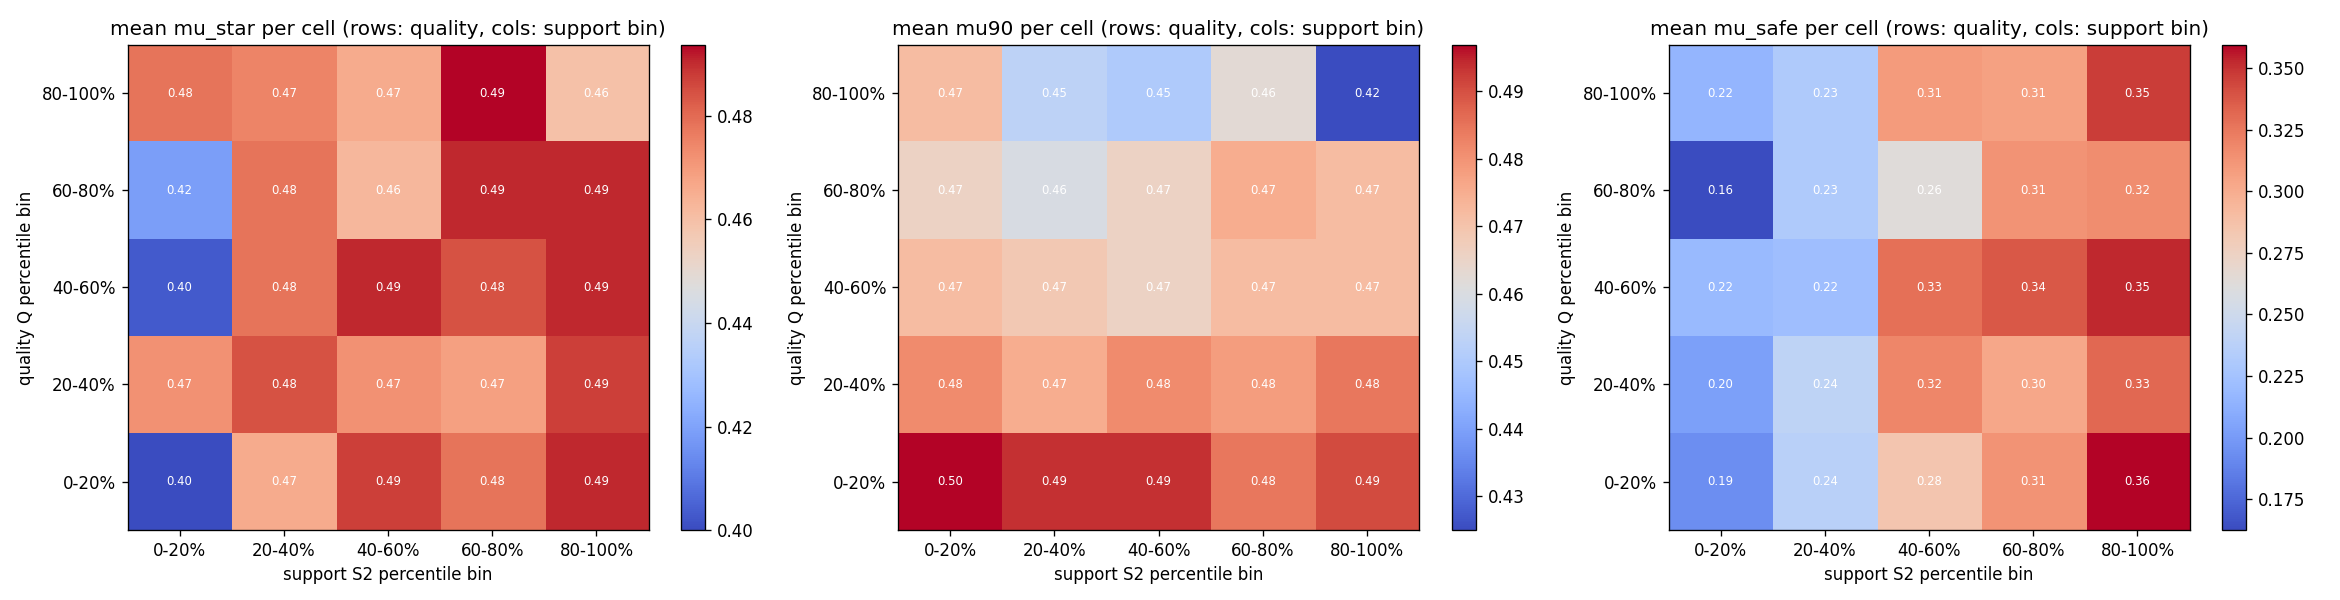
\includegraphics[width=0.85\linewidth]{main_best_mu_map.png}

\raggedright\small $\mu^{\text{safe}}$ by support quintile: \textbf{0.20, 0.23, 0.30, 0.31, 0.34} --- in every quality row. This curve is what we used to assign $\mu$ next.
\end{frame}

% =============================================================================================
\section{Assigning mu}
\begin{frame}[shrink=3]{Experiment A: assigning $\mu$ by support quintile}
\small
\begin{tabularx}{\linewidth}{lY}
\toprule
Source windows & \textbf{161{,}291} random windows ($\times31\approx5$M generated transitions). \textbf{Same windows in every condition}; only $\mu$ differs.\\
Support & $S_2$ reconstruction score, quintiles within these windows\\
RL & TD3+BC (CORL), batch 1024, 1M steps, 3 seeds; score = mean of last 5 evals\\
\bottomrule
\end{tabularx}
\vspace{0.4em}

\centering
\begin{tabular}{lcccccc}
\toprule
condition & \multicolumn{5}{c}{$\mu$ per support quintile (low $\to$ high)} & mean\\
\midrule
\cond{none} & \multicolumn{5}{c}{original data only} & --\\
\cond{uniform\_0.3} & 0.3 & 0.3 & 0.3 & 0.3 & 0.3 & 0.3\\
\cond{adaptive} & 0.20 & 0.25 & 0.30 & 0.35 & 0.40 & 0.3\\
\cond{inverted} & 0.40 & 0.35 & 0.30 & 0.25 & 0.20 & 0.3\\
\midrule
\cond{uniform\_0.5} & 0.5 & 0.5 & 0.5 & 0.5 & 0.5 & 0.5\\
\cond{adaptive\_wide} & 0.3 & 0.4 & 0.5 & 0.6 & 0.7 & 0.5\\
\cond{inverted\_wide} & 0.7 & 0.6 & 0.5 & 0.4 & 0.3 & 0.5\\
\bottomrule
\end{tabular}

\raggedright\scriptsize \cond{adaptive} follows the $\mu^{\text{safe}}$ curve. \cond{inverted} uses the same values in the wrong order: controls for mixing $\mu$ values. Rule: \yes{} if adaptive beats \emph{both} same-mean controls (Welch, $p<0.05$).
\end{frame}

\begin{frame}[shrink=3]{Experiment A results: two TD3+BC implementations}
\centering
\small
\begin{tabular}{@{}lccc@{}}
\toprule
condition & PyTorch (CORL) & JAX port & data: dyn.\ MSE / gain\\
\midrule
\cond{none} & $48.65\pm0.18$ & $48.72\pm0.06$ & --\\
\cond{uniform\_0.3} & $51.02\pm0.66$ & $51.51\pm0.36$ & 0.0096 / 0.057\\
\cond{adaptive} & $\mathbf{53.53\pm0.37}$ & $\mathbf{54.91\pm0.41}$ & 0.0090 / 0.079\\
\cond{inverted} & $51.72\pm0.49$ & $51.81\pm0.60$ & 0.0091 / 0.083\\
\midrule
\cond{uniform\_0.5} & $\mathbf{58.67\pm0.45}$ & $\mathbf{59.31\pm0.30}$ & 0.0076 / 0.327\\
\cond{adaptive\_wide} & -- & $58.60\pm0.65$ & 0.0092 / 0.220\\
\cond{inverted\_wide} & -- & $58.81\pm0.70$ & 0.0075 / 0.319\\
\bottomrule
\end{tabular}
\vspace{0.4em}

\raggedright
\begin{tabular}{@{}lll@{}}
\toprule
comparison & PyTorch & JAX\\
\midrule
adaptive $-$ uniform\_0.3 & $+2.51$ ($p=0.009$) & $+3.40$ ($p<0.001$)\\
adaptive $-$ inverted & $+1.81$ ($p=0.009$) & $+3.10$ ($p=0.003$)\\
adaptive $-$ uniform\_0.5 & $-5.14$ ($p<0.001$) & $-4.40$ ($p<0.001$)\\
adaptive\_wide $-$ uniform\_0.5 & -- & $-0.71$ ($p=0.20$)\\
adaptive\_wide $-$ inverted\_wide & -- & $-0.21$ ($p=0.72$)\\
\bottomrule
\end{tabular}
\end{frame}

\begin{frame}[shrink=6]{Experiment A: learning curves (JAX)}
\centering
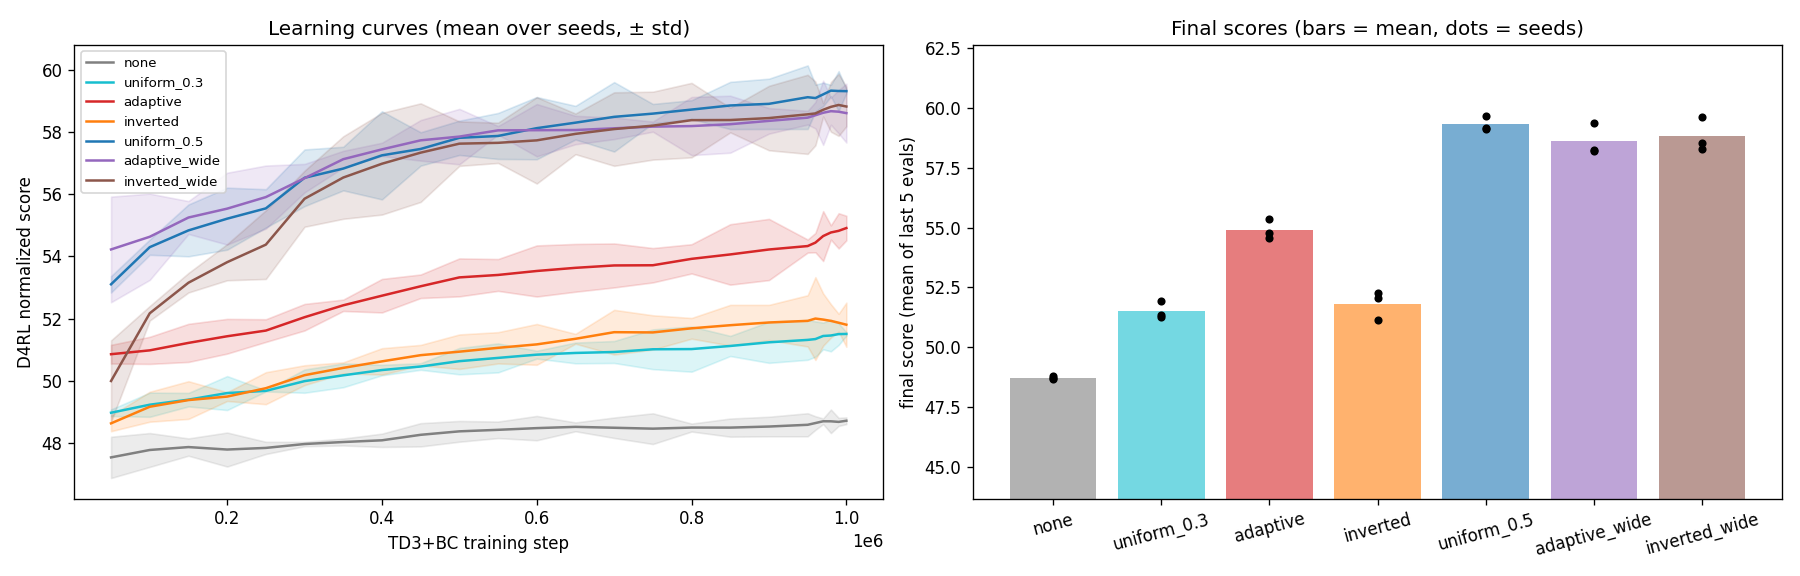
\includegraphics[width=\linewidth]{rl_jax.png}

\raggedright\small
\begin{itemize}
\item At mean $\mu=0.3$: support-adaptive is clearly better than both controls, \textbf{replicated} across two implementations (H2c \yes).
\item At mean $\mu=0.5$: no benefit. Pushing high-support windows to $\mu=0.7$ \emph{raises} physics error (0.0092 vs 0.0076) and lowers gain.
\item Consistent with the window study: the support effect is strongest at $\mu\approx0.2$--$0.35$ and vanishes near 0.5.
\end{itemize}
\end{frame}

% =============================================================================================
\section{Assigning alpha}
\begin{frame}{From $\mu$ to $\alpha$: design}
\small
Since $\mu$-adaptation did not help at $\mu=0.5$, we fixed $\mu=0.5$ and varied the \textbf{return multiplier} instead.
\vspace{0.3em}

\begin{tabularx}{\linewidth}{lY}
\toprule
Data & 32{,}258 windows (subset of the 161k, seed 2) $\Rightarrow$ 1M generated transitions; JAX TD3+BC, 1M steps\\
Stage 1 & global $\alpha\in\{1.0,1.1,1.3,1.5,1.8,2.0\}$, 3 seeds $\Rightarrow$ best $\alpha^*$\\
Stage 2 & $\alpha$ by $S_2$ quintile around $\alpha^*$: \cond{alpha\_up} $=1.1,1.2,1.3,1.4,1.5$ (low$\to$high support), \cond{alpha\_down} reversed; 8 seeds\\
Stage 3 & control: \cond{alpha\_random} uses the same five values assigned \emph{at random}; fresh seeds 10--14\\
\bottomrule
\end{tabularx}
\vspace{0.4em}

\textbf{Reading:} if \cond{alpha\_up} $>$ \cond{alpha\_random}, support matters. If \cond{alpha\_random} $\approx$ \cond{alpha\_up} $>$ uniform, only \emph{mixing} $\alpha$ values matters.
\end{frame}

\begin{frame}[shrink=2]{$\alpha$ results: Stage 1 and 2}
\begin{columns}[T]
\begin{column}{0.58\linewidth}
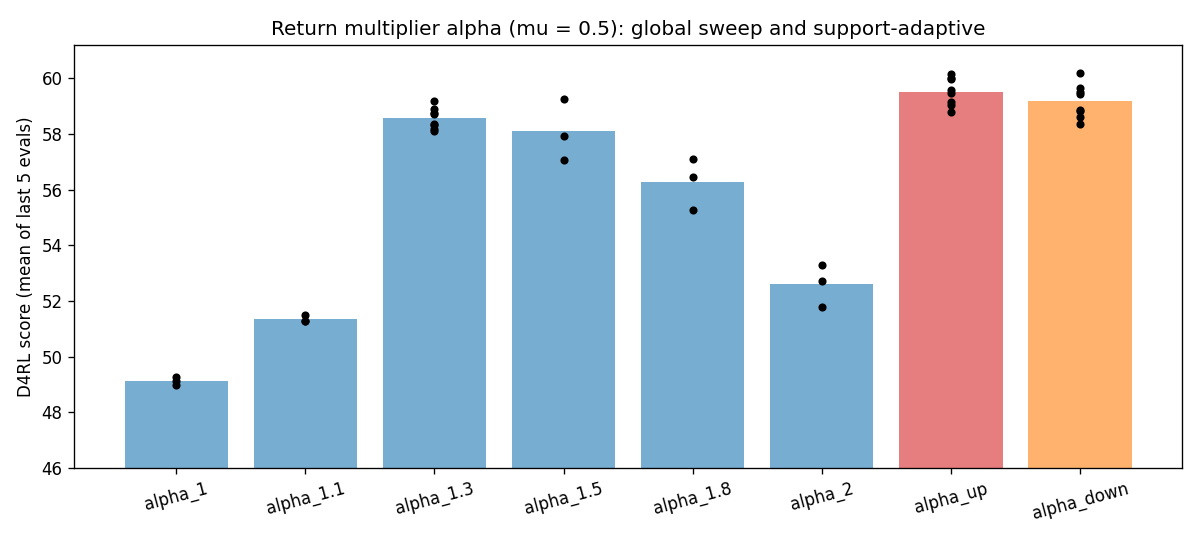
\includegraphics[width=\linewidth]{alpha_bars.png}
\end{column}
\begin{column}{0.40\linewidth}
\footnotesize
\begin{tabular}{@{}lrr@{}}
\toprule
condition & score & seeds\\
\midrule
$\alpha=1.0$ & $49.14\pm0.14$ & 3\\
$\alpha=1.1$ & $51.35\pm0.14$ & 3\\
$\alpha=1.3$ & $\mathbf{58.57\pm0.38}$ & 8\\
$\alpha=1.5$ & $58.10\pm1.10$ & 3\\
$\alpha=1.8$ & $56.28\pm0.93$ & 3\\
$\alpha=2.0$ & $52.61\pm0.77$ & 3\\
\midrule
\cond{alpha\_up} & $\mathbf{59.53\pm0.51}$ & 8\\
\cond{alpha\_down} & $59.18\pm0.62$ & 8\\
\bottomrule
\end{tabular}
\end{column}
\end{columns}
\vspace{0.3em}
\small
\begin{itemize}
\item Interior optimum at $\alpha=1.3$ (matches the paper). $\alpha=1$ ($\approx$ no guidance push) is barely better than no augmentation.
\item up $-$ 1.3: $+0.96$ ($p=0.001$); down $-$ 1.3: $+0.61$ ($p=0.035$); up $-$ down: $+0.35$ ($p=0.24$).
\item Both directions help $\Rightarrow$ suspect it is the \emph{mix}, not the support ordering.
\end{itemize}
\end{frame}

\begin{frame}{$\alpha$ results: Stage 3 (random-mix control)}
\begin{columns}[T]
\begin{column}{0.55\linewidth}
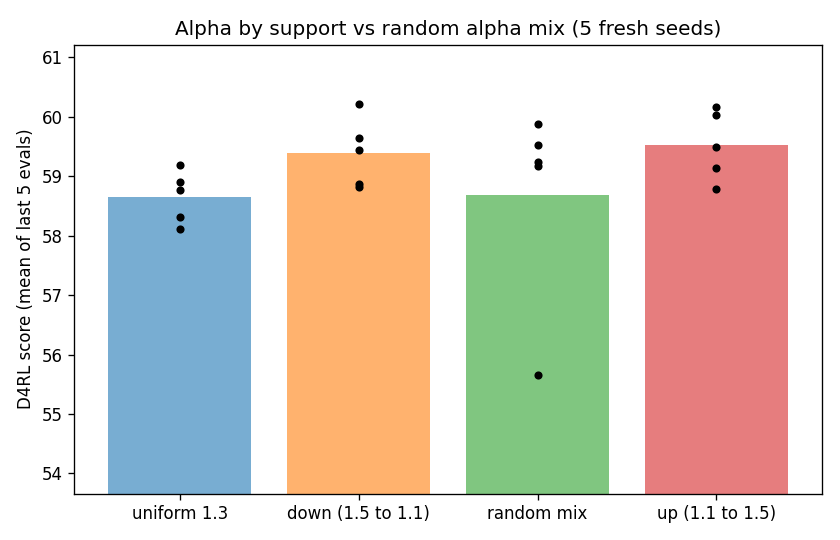
\includegraphics[width=\linewidth]{alpha_stage3_bars.png}
\end{column}
\begin{column}{0.43\linewidth}
\footnotesize
\begin{tabular}{@{}lr@{}}
\toprule
condition (5 fresh seeds) & score\\
\midrule
$\alpha=1.3$ & $58.66\pm0.44$\\
\cond{alpha\_down} & $59.40\pm0.58$\\
\cond{alpha\_random} & $58.69\pm1.72$\\
\cond{alpha\_up} & $59.52\pm0.58$\\
\bottomrule
\end{tabular}
\vspace{0.4em}

\begin{itemize}
\item up $-$ random: $+0.83$ ($p=0.35$)
\item up $-$ down: $+0.12$ ($p=0.74$)
\item up $-$ 1.3: $+0.87$ ($p=0.031$)
\item random $-$ 1.3: $+0.04$ ($p=0.97$)
\end{itemize}
\end{column}
\end{columns}
\vspace{0.4em}
\small
\textbf{Reading:} \cond{alpha\_up} reliably beats uniform $\alpha=1.3$ (replicated on fresh seeds), but cannot be separated from the random mix (high variance, 1.72) or from \cond{alpha\_down}. Evidence that the support \emph{ordering} matters for $\alpha$: \textbf{inconclusive}.
\end{frame}

% =============================================================================================
\section{Learned map}
\begin{frame}{Learning continuous $\mu(S,Q)$ and $\alpha(S,Q)$}
\small
Instead of hand-picked quintile maps, a smooth map with 6 parameters:
\[
\mu_i=0.3+0.4\,\sigma(a_0+a_S S'_i+a_Q Q'_i),\qquad
\alpha_i=1.0+0.8\,\sigma(c_0+c_S S'_i+c_Q Q'_i)
\]
$S',Q'\in[-\tfrac12,\tfrac12]$ centred percentiles; $\mu\in[0.3,0.7]$, $\alpha\in[1.0,1.8]$. Per-window $\mu$ implemented by noising each window at its own $\sigma_{k_0(i)}$ inside one batched sampler.
\vspace{0.4em}

\begin{tabularx}{\linewidth}{lY}
\toprule
Optimiser & CMA-ES on the D4RL score (black box)\\
global search & only $[a_0,c_0]$ (best single $\mu,\alpha$): 13 candidates\\
learned search & all 6 parameters: 43 candidates\\
Search budget & 16{,}129 windows (500k transitions), 2 seeds; common random numbers across candidates\\
Confirmation & 1M transitions, 5 \textbf{fresh} seeds (20--24); rule: learned must beat best global ($p<0.05$)\\
\bottomrule
\end{tabularx}
\end{frame}

\begin{frame}{Learned map: search and what it found}
\centering
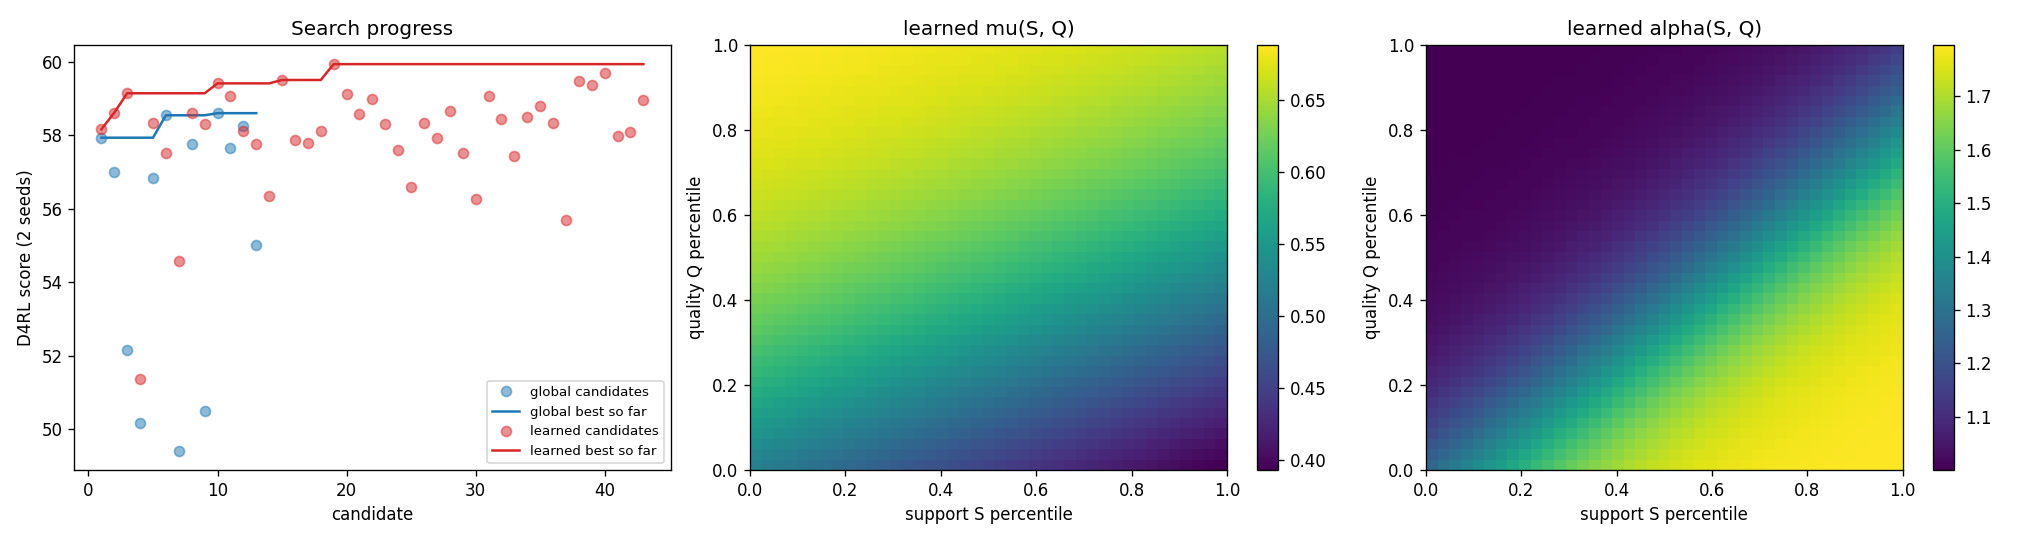
\includegraphics[width=\linewidth]{search.png}

\raggedright\small
\begin{itemize}
\item Best learned (search): 59.93 vs 58.60 for best global --- but on only 2 seeds and selected from 43 candidates.
\item Learned $\mu$: \emph{decreases} with support, increases with quality ($a_S=-1.4$, $a_Q=+3.3$) --- opposite of H2a/H2b.
\item Learned $\alpha$: strongly up with support, down with quality ($c_S=+6.2$, $c_Q=-7.0$): push hard only well-supported, low-quality windows.
\end{itemize}
\end{frame}

\begin{frame}{Learned map: confirmation on fresh seeds}
\begin{columns}[T]
\begin{column}{0.45\linewidth}
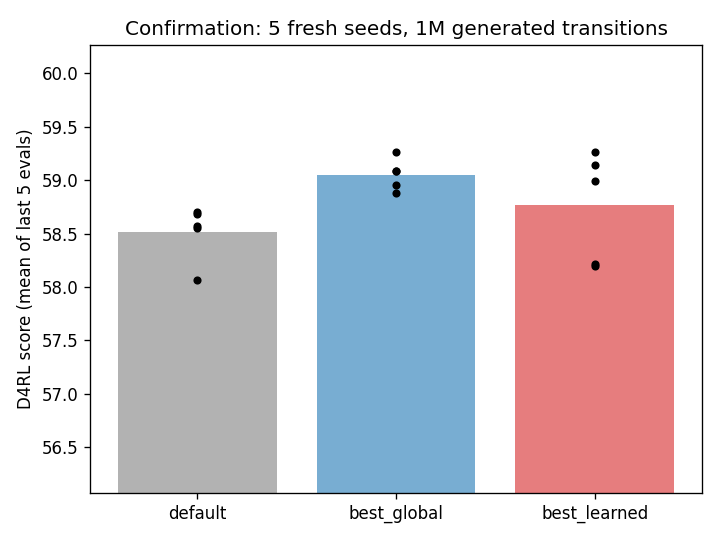
\includegraphics[width=\linewidth]{confirm_bars.png}
\end{column}
\begin{column}{0.53\linewidth}
\scriptsize
\begin{tabular}{@{}lccc@{}}
\toprule
setting & score (5 seeds) & mean $\mu$ & mean $\alpha$\\
\midrule
default & $58.51\pm0.26$ & 0.500 & 1.300\\
best global & $\mathbf{59.05\pm0.15}$ & 0.565 & 1.356\\
best learned & $58.76\pm0.52$ & 0.592 & 1.277\\
\bottomrule
\end{tabular}
\vspace{0.5em}

\small
\begin{itemize}
\item learned $-$ global: $-0.29$ ($p=0.29$) $\Rightarrow$ \nope.
\item global $-$ default: $+0.54$ ($p=0.006$): a slightly larger single $\mu,\alpha$ helps.
\item Search advantage was a winner's curse (2 seeds, 43 tries).
\item Learned data has higher physics error (0.0091 vs 0.0066).
\end{itemize}
\end{column}
\end{columns}
\end{frame}

% =============================================================================================
\section{Follow-up tests}
\begin{frame}{H3: is the diffusion model needed at all?}
\begin{columns}[T]
\begin{column}{0.5\linewidth}
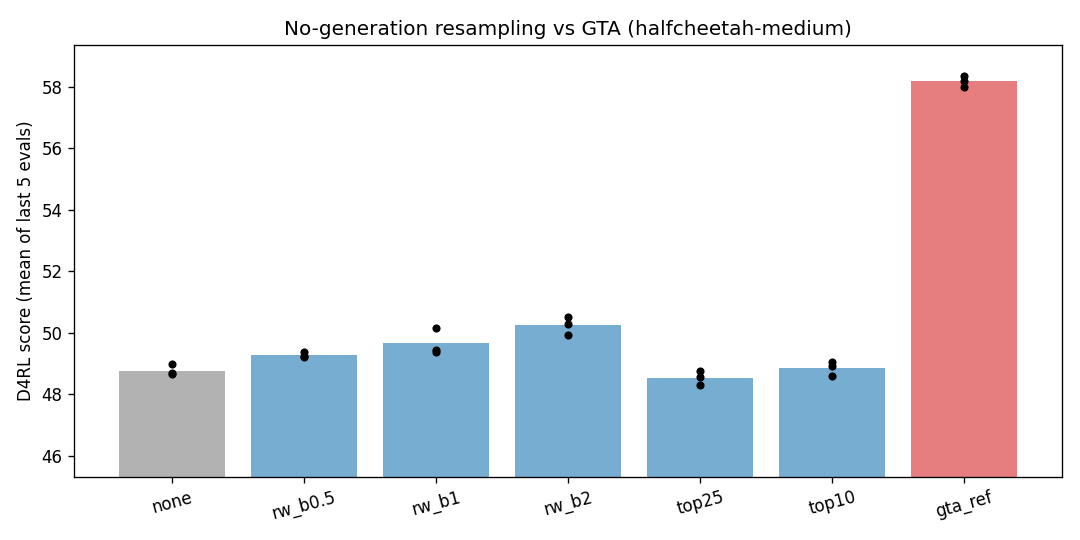
\includegraphics[width=\linewidth]{h3_bars.png}
\end{column}
\begin{column}{0.48\linewidth}
\scriptsize
5M extra transitions \emph{resampled} from the original data (no generation):
\vspace{0.3em}

\begin{tabular}{@{}lrr@{}}
\toprule
condition & score & \% of GTA gain\\
\midrule
none & $48.77$ & 0\\
reward-weighted $\beta=0.5$ & $49.27$ & 5\\
reward-weighted $\beta=1$ & $49.66$ & 9\\
reward-weighted $\beta=2$ & $50.24$ & 16\\
top-25\% windows & $48.53$ & $-3$\\
top-10\% windows & $48.85$ & 1\\
GTA ($\mu$ 0.5, $\alpha$ 1.3) & $\mathbf{58.18}$ & 100\\
\bottomrule
\end{tabular}
\end{column}
\end{columns}
\vspace{0.4em}
\small Reweighting existing data recovers at most 16\% of GTA's gain: the gain comes from \textbf{new, higher-reward} states, not from re-emphasising good ones.
\end{frame}

\begin{frame}{H4/H5: can a cheaper editor (VAE) replace diffusion?}
\small
\textbf{H4:} return-conditioned VAE edits windows in latent space (1{,}000-window simulator check; GTA ref: $+32\%$, dyn.\ MSE 0.0075).
\vspace{0.2em}

\centering\footnotesize
\begin{tabular}{@{}lrrrr@{}}
\toprule
method & gain & dyn.\ MSE & shift & TD3+BC\\
\midrule
VAE reconstruction & $+0.5\%$ & 0.032 & 0.21 & --\\
VAE edit $\alpha=1.3$, $\lambda=1$ & $+27.8\%$ & 0.046 & 0.39 & $48.51$ (3 seeds)\\
VAE edit $\alpha=1.5$, $\lambda=1$ & $+43.9\%$ & 0.087 & 0.61 & --\\
GTA $\mu=0.5$, $\alpha=1.3$ & $+32\%$ & \textbf{0.0075} & 0.89 & $\mathbf{58.5}$\\
\bottomrule
\end{tabular}
\vspace{0.4em}

\raggedright\small
\textbf{H5:} keep VAE-edited actions, roll out states with a learned dynamics ensemble: physics is consistent but reward \textbf{drops} ($-10$ to $-26\%$).
\vspace{0.3em}

\textbf{Reading:} the VAE gains reward but with $6\times$ the physics error, and TD3+BC gets nothing from it ($48.5$ = no augmentation). Physical validity matters more than reward gain.
\end{frame}

\begin{frame}{H6: trust-weighting generated transitions (Gate 0, oracle)}
\begin{columns}[T]
\begin{column}{0.5\linewidth}
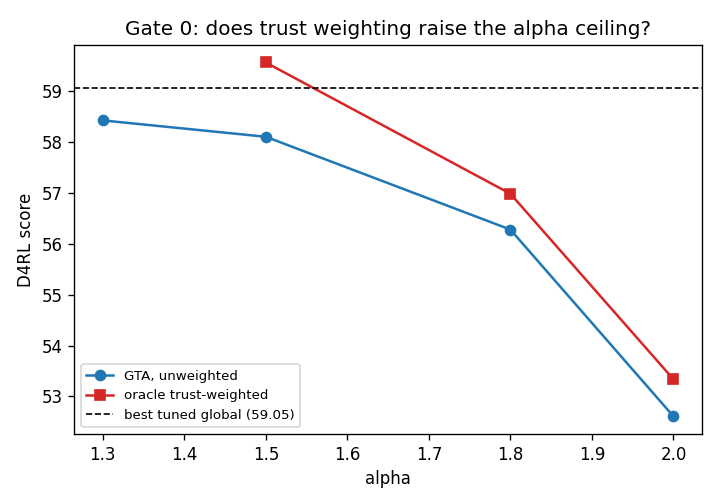
\includegraphics[width=\linewidth]{gate0.png}
\end{column}
\begin{column}{0.48\linewidth}
\small
Weight per generated transition $w=\exp(-\text{err}/0.0085)$ with the \emph{true} physics error (oracle); original data weight 1.
\vspace{0.3em}

\footnotesize
\begin{tabular}{@{}lrrr@{}}
\toprule
$\alpha$ & unweighted & weighted & $p$\\
\midrule
1.5 & $58.10$ & $\mathbf{59.56}$ & 0.13\\
1.8 & $56.28$ & $56.98$ & 0.32\\
2.0 & $52.61$ & $53.34$ & 0.29\\
\bottomrule
\end{tabular}
\end{column}
\end{columns}
\vspace{0.4em}
\small
Gate passed: best weighted score 59.56 exceeds best tuned global (59.05). Differences individually not significant (3 seeds). Next: replace the oracle with a learned error estimate (e.g.\ the $S_2$ score of the \emph{edited} window).
\end{frame}

\begin{frame}{H7: does a simple bound explain the $\alpha$ optimum?}
\begin{columns}[T]
\begin{column}{0.5\linewidth}
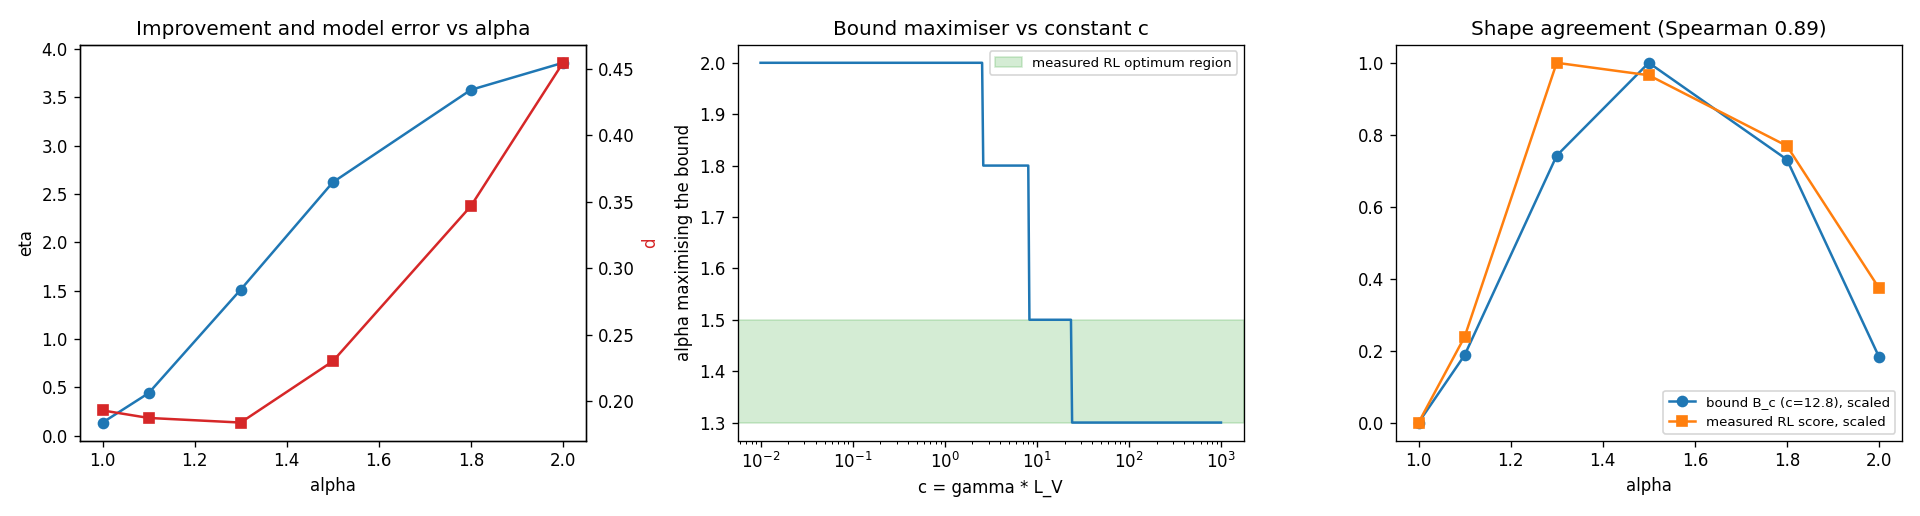
\includegraphics[width=\linewidth]{t1.png}
\end{column}
\begin{column}{0.48\linewidth}
\small
\[
B_c(\alpha)=\frac{\eta(\alpha)-c\,d(\alpha)}{1-\gamma}
\]
$\eta$: true reward gain per step; $d$: next-state error; $c=\gamma L_V$.
\vspace{0.3em}

\footnotesize
\begin{tabular}{@{}lrrr@{}}
\toprule
$\alpha$ & $\eta$ & $d$ & RL score\\
\midrule
1.0 & 0.136 & 0.193 & 49.14\\
1.3 & 1.511 & 0.184 & \textbf{58.42}\\
1.5 & 2.621 & 0.230 & 58.10\\
2.0 & 3.858 & 0.455 & 52.61\\
\bottomrule
\end{tabular}
\end{column}
\end{columns}
\vspace{0.4em}
\small Any $c\in[8.3,10^3]$ (incl.\ the worst-case 824) puts the maximiser at $\alpha=1.3$--$1.5$; best rank fit $\rho=0.89$. Explanatory only ($c$ fitted on one dataset): $\alpha$ trades reward gain against physics error, the same trade-off support measures.
\end{frame}

% =============================================================================================
\section{Conclusions}
\begin{frame}[shrink=26]{Scorecard}
\small
\renewcommand{\arraystretch}{1.15}
\begin{tabularx}{\linewidth}{@{}p{0.34\linewidth}Yp{0.14\linewidth}@{}}
\toprule
claim & evidence & result\\
\midrule
Reconstruction score $S_2$ measures support & $\rho=0.79$ with kNN, $0.74$ with exact likelihood & \yes\\
H2a support $\Rightarrow$ safe $\mu$ & $\mu^{\text{safe}}$ $+0.18$ $[0.14,0.23]$; physics error vs $S$ at every $\mu$ & \yes\\
H2b quality $\Rightarrow$ lower $\mu$ & $\beta_Q\approx0$; quality only drives gain (ceiling) & \nope\\
H2c adaptive $\mu$, mean 0.3 & $+2.5$/$+3.4$ over controls, 2 implementations & \yes\\
H2c adaptive $\mu$, mean 0.5 & $-0.7$ ($p=0.20$) & \nope\\
$\alpha$ by support & beats uniform 1.3 ($+0.9$) but $\approx$ random mix & inconclusive\\
Learned $\mu(S,Q),\alpha(S,Q)$ & $-0.3$ vs tuned global ($p=0.29$) & \nope\\
H3 generation needed & resampling recovers $\le16\%$ & \yes\\
H4/H5 VAE editor & no RL gain; $6\times$ physics error & \nope\\
H6 trust weighting (oracle) & 59.56 vs 59.05 & gate passed\\
\bottomrule
\end{tabularx}
\vspace{0.3em}

\textbf{Takeaway:} support predicts edit damage; it pays off for small $\mu$. Best score so far: \textbf{59.5} ($\alpha$ mix / oracle weighting) vs 58.5 GTA default.
\end{frame}

\begin{frame}[shrink=10]{Limitations and next steps}
\small
\textbf{Limitations}
\begin{itemize}
\item One dataset (\texttt{halfcheetah-medium-v2}), one behaviour policy: support varies only moderately.
\item 3--5 seeds: differences below $\approx1$ point are hard to resolve (e.g.\ random $\alpha$ mix has std 1.7).
\item Guidance at $w=0$ instead of the paper's $w=2$; condition dropout active during sampling (upstream).
\item $\mu^{\text{safe}}$ and the wide/$\alpha$ designs were defined after earlier results (exploratory).
\end{itemize}
\vspace{0.4em}
\textbf{Next steps}
\begin{itemize}
\item Mixed-quality datasets (medium-replay, medium-expert) where support varies much more.
\item H6 with a learned, non-oracle trust weight (post-edit $S_2$ or dynamics-ensemble disagreement).
\item Quality-indexed $\mu$ (\cond{quality\_adaptive}/\cond{quality\_inverted}, already implemented, not yet run).
\item More seeds for the $\alpha$ up/random/down comparison.
\end{itemize}
\end{frame}

\begin{frame}{Reproducibility}
\scriptsize
\begin{tabularx}{\linewidth}{lY}
\toprule
command & produces\\
\midrule
\texttt{python scripts/h2\_run.py pool | sweep | analyze} & window-level study (\texttt{outputs/h2/})\\
\texttt{bash scripts/h2\_rl\_all.sh} & Experiment A, PyTorch (\texttt{outputs/h2\_rl/})\\
\texttt{bash scripts/h2\_rl\_jax\_all.sh}, \texttt{h2\_rl\_wide.sh} & Experiment A, JAX + wide (\texttt{outputs/h2\_rl\_jax/})\\
\texttt{bash scripts/h2\_alpha.sh}, \texttt{h2\_alpha\_stage3.sh} & $\alpha$ stages 1--3 (\texttt{outputs/h2\_alpha/})\\
\texttt{python scripts/h2\_learn.py run} & CMA-ES learned map (\texttt{outputs/h2\_learn/})\\
\texttt{bash scripts/h3\_nogen.sh}, \texttt{h4\_vae\_rl.sh}, \texttt{h6\_gate0.sh} & H3, H4, H6\\
\texttt{python scripts/h5\_vae\_dyn.py}, \texttt{h7\_t1.py} & H5, H7\\
\bottomrule
\end{tabularx}
\vspace{0.4em}

Checkpoint \texttt{model-1000000.pt} (EMA). Code: \texttt{src/h2/} (\texttt{support}, \texttt{analysis}, \texttt{rl\_data}, \texttt{learned}, \dots), \texttt{jax\_impl/}.
\end{frame}

\end{document}
